\subsection{Algorithm process}
Figure \ref{fig:pentos} shows the high level process of our algorithm. It first pick a best valid place to build the request building, which evaluated by several criterion. Then, build a best road to connect it to existing road or edges. If the request is a residence, there is an additional step to build company park and pond. The detailed illustration will be present in next subsection.

\begin{figure}
\center
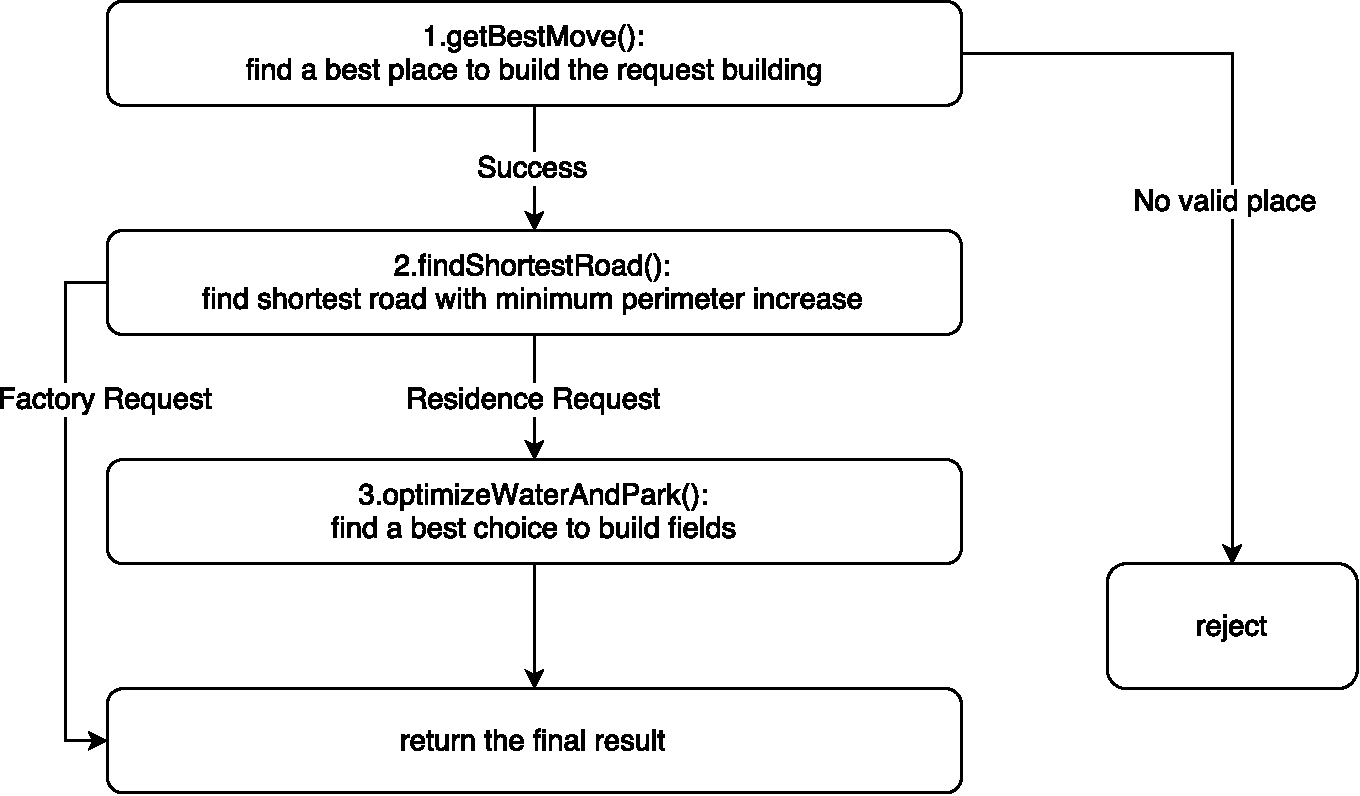
\includegraphics[scale=0.5]{pentos.pdf}
\caption{high level algorithm flow chart of our submitted approach}
\label{fig:pentos}
\end{figure}

\subsection{Building Placement}
This module is tend to find the best place to build the request building. The place must could be connected to an existing road or edges. Then, we try to defined the ``best" in several ways, which will be explained in each subsubsection.
\subsubsection{global: row-by-row}
This is a naive global strategy that we try first. The residences are build row by row from top to bottom, which means each time find the buildable place with the lowest row index. The factories are build row by row from bottom to top, which means each time find the buildable place with the highest row index. The idea behind this approach is that separate the residences and factories to avoid gaps between adjacent residence and factory, as the residence cannot build next to factory.

Using this naive approach, we can get around 1600~1700 score. The implementation of the naive strategy help us more understand the game at the beginning. Later, we switched to other strategies.
\subsubsection{global: diagonal}
This is another global strategy. The residences are build from left-up corner to right-down corner, which means each time find the buildable place with the lowest sum of row index plus column index. The factories are build from right-down corner to left-up corner, which means each time find the buildable place with the highest sum of row index plus column index. The idea behind this approach is still try to separate the residences and factories. But the diagonal gap could be more flexible, that each time there are more different buildable places.

In addition to the global diagonal pattern, we add another small features to the selection process. For the candidate spaces that have roughly same value of $(i+j)$, which is denotes the sum of row index and column index, we pick the one has minimum $(i-j)$, which means most close to the diagonal line. The idea behind this feature is to make the frontier of residences and factories more convex. Because the waste value of building near the edge is always less, we prefer to preserve the spaces near the edge when there is also another good choice more near the diagonal.
\subsubsection{global: housing at center, factories on edges}
This is a different global strategy we have tried. In this strategy, we build factories from edges to center and build residences from center to edges. The idea behind it is that the factories are more regular in shape that can fit very well on the edges, while residences have more various shapes. But the experiments told us this is not a good strategy, so we give up it later. The reason we speculate is that the factories are easy to build nearly perfect compact. But build all factories near the edges makes the gap between factories and residences longer, and increase the difficulties of building roads.
\subsubsection{perimeter}
Finally, we use diagonal strategy as our global strategy. But add perimeter to be the most significant key to evaluate candidate locations. For a candidate location, some of its cells is neighbor to an already occupied cell in the map, some of its cells is neighbor to an vacant cell in the map. The algorithm count the number of cells that neighbor to an already occupied cell, which called the perimeter of this location. Then we choose the one with largest perimeter. The idea behind it is the larger perimeter means the buildings are more compact. And, it has been shown that perimeter evaluation made an significant contribution to our good performance.

As a summary, in the submitted version, we use diagonal global strategy and perimeter local strategy. When compare different choices, we use the perimeter as the first key, $(i+i)$ as the second key, and $(i-j)$ as the third key.
\subsubsection{number of components}
Besides the submitted version, we have tried another feature to choose the best place. In the last subsubsection, we mentioned the number of cells that neighbor to already occupied cell. It generally makes the buildings compact, but sometimes cause small closed area that lower the land use efficiency. so we consider another measurement called number of components. It is defined as the number of connected vacant spaces components that neighbor to the current candidates place. The idea is split vacant components as less as possible. Figure \ref{fig: numComponents} shows the idea more intuitively.

\begin{figure}
\center
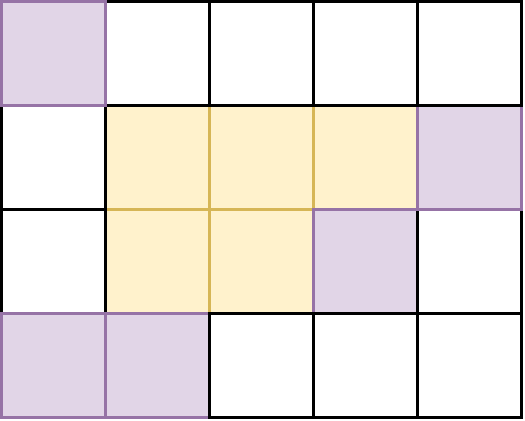
\includegraphics[scale=0.5]{numComponents.pdf}
\caption{
Suppose the yellow grids denote the candidate building place,
the purple grids denote already occupied cells,
the white grids denote vacant cells.
Then the number of components in this example is 3.}
\label{fig: numComponents}
\end{figure}

In our experiments, whatever we put the number of components as the first key or second key, the performance decrease a little. So finally we removed this feature.

